Fissato il valore della tensione $V_{DS}$, la $I_{on}$ è definita come il valore di corrente di Drain $I_D$ che attraversa un MOSFET quando il valore della tensione $V_{GS}$ è massimo:

\begin{equation}
    I_{on}(V_{DS}) = \max_{V_{GS}} I_D(V_{DS},V_{GS})
\end{equation}

Per questo studio, si è interessati alla variazione percentuale di questo parametro al crescere della dose assorbita e successivamente all'\emph{annealing}. Il valore massimo di $V_{GS}$ considerato è il valore massimo utilizzato per le misure, ovvero $900 mV$. L'unica eccezione è il MOSFET a canale P di dimensioni 600-0.030, per il quale è stata considerata la $I_D$ a $V_{GS} = 700 mV$, poiché a $V_{GS} = 900mV$ lo strumento di misura satura. Alcuni risultati ottenuti sono mostrati nelle immagini \ref{fig:delta_I_on_vds_450_mv} ($V_{DS} = 450 mV$) e \ref{fig:delta_I_on_vds_900_mv} ($V_{DS} = 900 mV$).

%Vds = 450 mA 
\begin{figure}[h]
    \centering
    % W = 100 
    \includegraphics[width=0.49\textwidth]{./capitolo2/I_on/NMOS/Vds_450_mV/Delta_i_on_W_100.png}
    \includegraphics[width=0.49\textwidth]{./capitolo2/I_on/PMOS/Vds_450_mV/Delta_i_on_W_100.png}\\
    \vspace{0.2cm}
    % W = 200
    \includegraphics[width=0.49\textwidth]{./capitolo2/I_on/NMOS/Vds_450_mV/Delta_i_on_W_200.png}
    \includegraphics[width=0.49\textwidth]{./capitolo2/I_on/PMOS/Vds_450_mV/Delta_i_on_W_200.png}\\
    \vspace{0.2cm}

    % W = 600
    \includegraphics[width=0.49\textwidth]{./capitolo2/I_on/NMOS/Vds_450_mV/Delta_i_on_W_600.png}
    \includegraphics[width=0.49\textwidth]{./capitolo2/I_on/PMOS/Vds_450_mV/Delta_i_on_W_600.png}

    \caption[Dati $\% \Delta I_{on}$ a $V_{DS}=450mV$ ]{$\% \Delta I_{on}$ calcolata nei dispositivi MOSFET a $V_{DS} = 450mV$ rispetto alle misure fatte prima di subire la dose di irraggiamento. A sinistra i dispositivi a canale N, a destra i dispositivi a canale P. I grafici sono raggruppati per larghezza di canale.}
    \label{fig:delta_I_on_vds_450_mv}

\end{figure}

%Vds = 900 mA
\begin{figure}[h]
    \centering
    % W = 100 
    \includegraphics[width=0.49\textwidth]{./capitolo2/I_on/NMOS/Vds_900_mV/Delta_i_on_W_100.png}
    \includegraphics[width=0.49\textwidth]{./capitolo2/I_on/PMOS/Vds_900_mV/Delta_i_on_W_100.png}\\
    \vspace{0.2cm}
    % W = 200
    \includegraphics[width=0.49\textwidth]{./capitolo2/I_on/NMOS/Vds_900_mV/Delta_i_on_W_200.png}
    \includegraphics[width=0.49\textwidth]{./capitolo2/I_on/PMOS/Vds_900_mV/Delta_i_on_W_200.png}\\
    \vspace{0.2cm}

    % W = 600
    \includegraphics[width=0.49\textwidth]{./capitolo2/I_on/NMOS/Vds_900_mV/Delta_i_on_W_600.png}
    \includegraphics[width=0.49\textwidth]{./capitolo2/I_on/PMOS/Vds_900_mV/Delta_i_on_W_600.png}

    \caption[Dati $\% \Delta I_{on}$ a $V_{DS}=900mV$ ]{$\% \Delta I_{on}$ calcolata nei dispositivi MOSFET a $V_{DS} = 900mV$ rispetto alle misure fatte prima di subire la dose di irraggiamento. A sinistra i dispositivi a canale N, a destra i dispositivi a canale P. I grafici sono raggruppati per larghezza di canale.}
    \label{fig:delta_I_on_vds_900_mv}

\end{figure}


Analizzando i grafici si possono ottenere diverse informazioni.
Per i MOSFET a canale N, la $I_{on}$ a basse dosi di irraggiamento aumenta leggermente (tra $0\%$ e $5\%$ del valore pre-irraggiamento), ma intorno ai $100 Mrad$ di \emph{TID} il valore diminuisce in maniera repentina. All'aumentare ulteriore dell'irraggiamento, il valore di $I_{on}$ cala in modo costante, ma lentamente. La stessa cosa succede dopo l'\emph{annealing}. Per i MOSFET a canale P, invece, il valore della $I_{on}$ cala in modo quasi lineare con l'irraggiamento, in maniera più consistente di quanto faccia per i dispositivi a canale N dopo i $100 Mrad$ di radiazioni subite. In seguito all'\emph{annealing}, il valore di $I_{on}$ nei PMOS aumenta notevolmente, senza però avvicinarsi al valore pre-irraggiamento. Queste variazioni sono coerenti con l'andamento della tensione di soglia dei dispositivi. 

Per i MOSFET a canale N, inoltre, il degrado della $I_{on}$ è più o meno consistente in base alla $V_{DS}$ a cui lo si misura. Infatti, le radiazioni hanno un effetto più evidente al crescere della tensione, causando una diminuzione percentuale maggiore. Ad esempio, per i MOSFET a canale N di lunghezza $180 nm$, passando da $V_{DS} = 450mA$ a $V_{DS} = 900 mA$, il valore di $\% \Delta I_{on}$ a $3 Grad$ di \emph{TID} aumenta di circa il $5\%$. Per i MOSFET a canale P, invece, la $\% \Delta I_{on}$ non è influenzata significativamente dal valore di $V_{DS}$.

Infine, anche la lunghezza del canale influenza la variazione di $I_{on}$. La differenza percentuale è tanto più negativa quanto più la lunghezza dei MOSFET è maggiore. Anche questo comportamento è coerente con quanto detto sulla tensione di soglia. Nei grafici è presente un'eccezione: la $\% \Delta I_{on}$ del MOSFET a canale P di dimensione 600-0.060 pare essere meno negativa rispetto a quella del MOSFET della stessa tipologia di dimensione 600-0.030. Quest'eccezione in realtà è dovuta alle modalità con cui è stata calcolata la $I_{on}$ per quest'ultimo dispositivo (vedi sopra).

\FloatBarrier


